\begin{frame}{Du transistor (1947) au \texttt{xeon} d'Intel}
    \begin{center}
        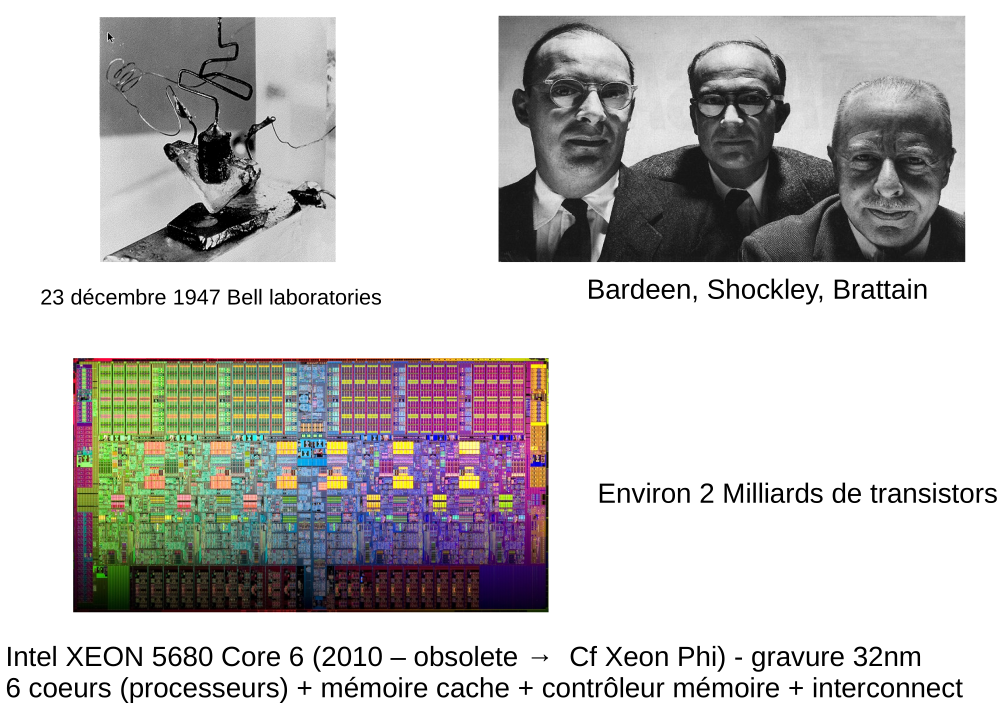
\includegraphics[scale=0.3]{./images/transistor_1947.png}
    \end{center}
\end{frame}

\begin{frame}{Jalons historiques: loi de Moore}
  \begin{columns}[T] % [T] aligne en haut, [c] centré, [b] en bas
    \begin{column}{0.5\textwidth}  % Colonne de gauche (50% de la largeur)
      \begin{itemize}
        \item Doublement du nombre de transistors tous les 18 mois.
      \end{itemize}
      \begin{center}
        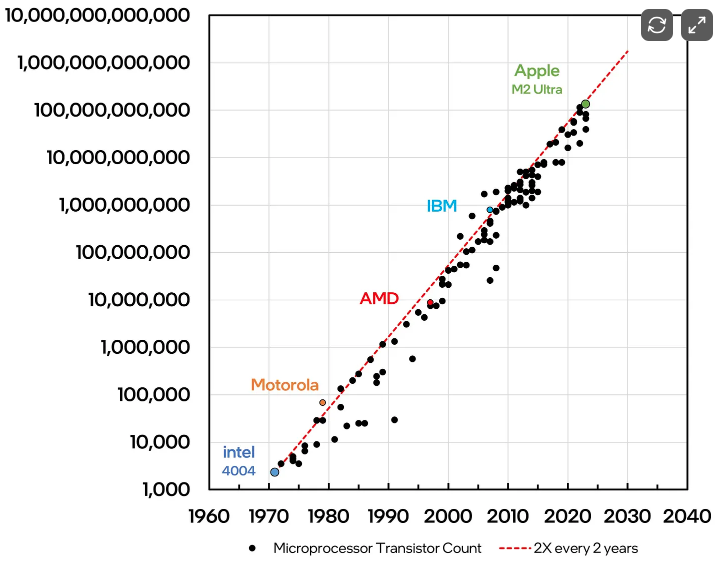
\includegraphics[scale=0.3]{./images/history_moore.png}
      \end{center}
    \end{column}

    \begin{column}{0.5\textwidth}  % Colonne de droite (50% de la largeur)
        \begin{itemize}
        \item Perspective historique plus large.
        \end{itemize}
        \begin{center}
          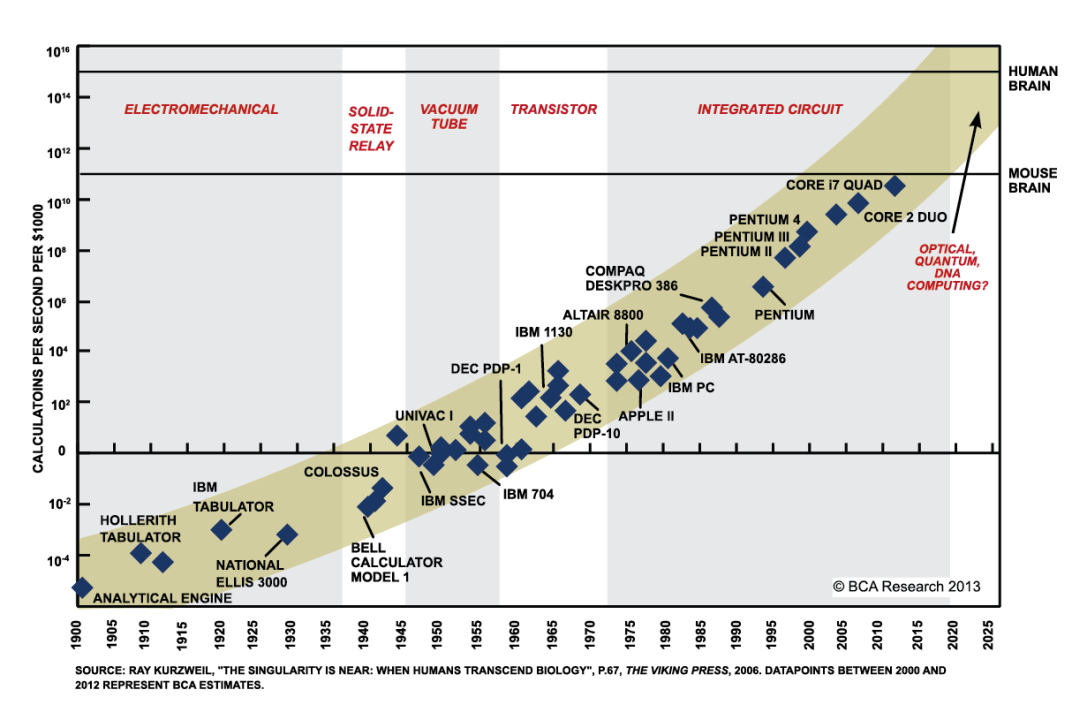
\includegraphics[scale=0.20]{./images/history_1.png}
        \end{center}
        1971 : Intel 4004
    \end{column}
    \end{columns}
\end{frame}

\begin{frame}{Le cas des mémoires :}
    \begin{center}
        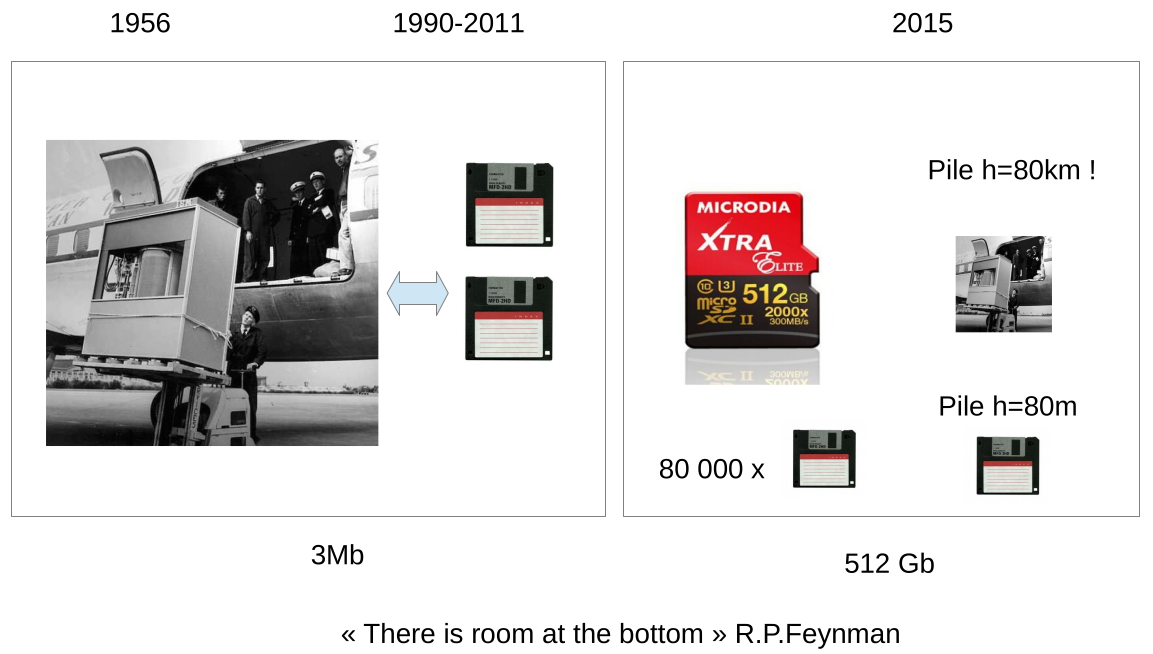
\includegraphics[scale=0.3]{./images/disquette.png}
    \end{center}
\end{frame}
